\documentclass[12pt,a4paper]{article}

\usepackage{graphicx}
 \usepackage{subfigure} 
 \usepackage[english]{babel}
 \usepackage[format=default,font=footnotesize,labelfont=bf]{caption}
\usepackage[ansinew]{inputenc} 		%Umlaute
\usepackage[T1]{fontenc} 				%Umlaute		
\usepackage[margin=1in]{geometry}		%Randabstand
\usepackage[onehalfspacing]{setspace}	%Zeilenabstand 1,5

\usepackage{floatflt}					%Umflossene Grafiken
\usepackage{float}
\usepackage[section]{placeins}
\usepackage{afterpage}
\usepackage{tabularx}

				%Highlight-boxen

\usepackage[framemethod=tikz]{mdframed}
\usepackage{lipsum}
\usepackage[many]{tcolorbox}

\newtcolorbox{myboxii}[1][]{
  breakable,
  freelance,
  title=#1,
  colback=white,
  colbacktitle=white,
  coltitle=black,
  fonttitle=\bfseries,
  bottomrule=0pt,
  boxrule=0pt,
  colframe=white,
  overlay unbroken and first={
  \draw[red!75!black,line width=3pt]
    ([xshift=5pt]frame.north west) -- 
    (frame.north west) -- 
    (frame.south west);
  \draw[red!75!black,line width=3pt]
    ([xshift=-5pt]frame.north east) -- 
    (frame.north east) -- 
    (frame.south east);
  },
  overlay unbroken app={
  \draw[red!75!black,line width=3pt,line cap=rect]
    (frame.south west) -- 
    ([xshift=5pt]frame.south west);
  \draw[red!75!black,line width=3pt,line cap=rect]
    (frame.south east) -- 
    ([xshift=-5pt]frame.south east);
  },
  overlay middle and last={
  \draw[red!75!black,line width=3pt]
    (frame.north west) -- 
    (frame.south west);
  \draw[red!75!black,line width=3pt]
    (frame.north east) -- 
    (frame.south east);
  },
  overlay last app={
  \draw[red!75!black,line width=3pt,line cap=rect]
    (frame.south west) --
    ([xshift=5pt]frame.south west);
  \draw[red!75!black,line width=3pt,line cap=rect]
    (frame.south east) --
    ([xshift=-5pt]frame.south east);
  },
}

\usepackage{fancyhdr}
\pagestyle{fancy}

\usepackage{listings}				%Codelisting
\usepackage{courier}
\usepackage{color}
\usepackage{acronym}				%Abk�rzungen
 
\definecolor{codegreen}{rgb}{0,0.6,0}
\definecolor{codegray}{rgb}{0.5,0.5,0.5}
\definecolor{codepurple}{rgb}{0.58,0,0.82}
\definecolor{backcolour}{rgb}{0.98,0.98,0.98}
 
\lstdefinestyle{mystyle}{
    backgroundcolor=\color{backcolour},   
    commentstyle=\color{codegreen},
    keywordstyle=\color{magenta},
    numberstyle=\tiny\color{codegray},
    stringstyle=\color{blue},
    basicstyle=\footnotesize,
    breakatwhitespace=false,         
    breaklines=false,                 
    captionpos=b,                    
    keepspaces=true,                 
    numbers=left,                    
    numbersep=5pt,                  
    showspaces=false,                
    showstringspaces=false,
    showtabs=false,                  
    tabsize=2
}
 
\lstset{style=mystyle}


\fancyfoot{}
\fancyfoot[R]{\thepage}

\usepackage{hyperref}
\usepackage{multibib} 
\newcites{Refs,Urls}{Literaturverzeichnis,Verzeichnis der Webadressen}

\usepackage{url}

\begin{document}

%==================Deckblatt===========================%
\ \vspace{0.1cm} 
\begin{center} 

\begin{huge} 
Bachelorthesis \\ 
\end{huge}
\ \\
\vspace{1cm} 

\noindent\rule{16cm}{-2em} 
\hrule\par\rule[-1em]{0pt}{2.5em}
\begin{large}
\textbf{Development of a Web-Application\\
for executing Job-Scripts on an IBM-Mainframe\\
in the context of Education\\}
\vspace{0.3cm}
\end{large}
\hrule\par\rule{0pt}{2em}
\ \\
\vspace{1cm} 


\begin{small}
Bachelorarbeit gem�� � 17 der Allgemeinen Pr�fungsordnung vom 01.08.2008 \\
im Bachelorstudiengang Informationsmanagement und Unternehmenskommunikation \\
an der Hochschule f�r angewandte Wissenschaften Neu-Ulm \\
\end {small}

\vspace{3cm} 


\end {center}

\begin{table} [!h]
\begin{tabular}{lll}

	Erstkorrektor	& 	&	Prof. Dr. Phillipp Brune \\
	Betreuer 		& 	&	Dr. Kevin Henrichs \\
	 & & \\
	Verfasser		&	&	Marc Morschhauser (Matr.-Nr.: 204041)\\
	 & & \\
	  & & \\
	   & & \\
	Thema erhalten & & 01.01.2020 \\
	Arbeit abgegeben & & 01.05.2020 \\

\end{tabular}
\label{tab:threecols}
\end{table}


\vspace{3cm} 
\noindent\rule{7.5cm}{1pt}\hspace{1cm}\noindent\rule{7.5cm}{1pt}
\hspace*{1cm}Unterschrift des Studierenden\hspace{2.7cm}Unterschrift und Firmenstempel der \\
\hspace*{10.5cm}Ausbildungsstelle
\thispagestyle{empty}
\newpage
%==================Ende Deckblatt===========================%
\begin{center}
In association with:
\vspace{1.5cm}
\begin{figure}[h]
	\centering
	
\includegraphics[scale=0.25]{img/Logos.jpg}
\end{figure}

\end{center}
\thispagestyle{empty}
\newpage
%==================Ende Logos===========================%

\pagenumbering{Roman}

\section{Abstract}
Hier kommt der/die/das Abstract.\\

\newpage

\listoffigures

\newpage
\section{List of abbreviations}
\begin{acronym}[Bash]
	 \acro{IoT}{Internet of Things}
	 \acro{I/O}{Input / Output}
 	 \acro{OS}{Operating System}
	 \acro{ULE}{Ubiquitous Learning Environment}
	 \acro{JCL}{Job Control Language}
 	 \acro{JES}{Job Entry Subsystem}
 	 \acro{OLTP}{Online Transaction Processing}
	 \acro{LPAR}{Logial Partitions}
	\acro{LAN}{Local Area Network}
	\acro{FTP}{File Transfer Protocol}
	\acro{SSH}{Secure Shell}
	\acro{SFTP}{Secure File Transfer Protocol}
\end{acronym}

\newpage

\tableofcontents

\newpage

\pagenumbering{arabic}




%===========Main Content=========%
\setcounter{page}{3}
%\begin{onehalfspacing}

\newpage

\section{Introduction}
Big Data, Cloud, Blockchain, \ac{IoT}  - Digitalization is steadily proceeding and with it the amount of data that has to be processed every day. Many web-services at this point are dependent on flexibility in first place. Big server farms facilitate an unprecedented agility to operators of online-businesses referring to their resource-planning. Urgent situations with high data traffic can be handled by adding physical or also virtual servers within minutes. However there are services where minutes make the difference between millions of euros. Those services demand for information technology, which not only has a high data throughput but also ensures the highest availability. The IBM Mainframe in its newest construction provides an \ac{I/O} of 288GB per second  while being available 99,999\% of the time running. This makes the Mainframe a cornerstone in present finance-sector's IT-management. Due to it's security and it's high speed it also finds it's use in other big industries - thus also insurances, the aerospace industry or big retail companies benefit from this supercomputer.\\
But since the IT improved considerably over the last decades, the Mainframe was presumed dead and many companies discontinued training their staff to maintain this technology. Contrary to their expectations they are dependent on it till today and they will presumably be in the remote future. What is left is a big gap in the division of skilled professionals that is hard to close.\\
The Goethe-University in Frankfurt, Germany, attends to participate in closing this gap. Therefore the university procured one of the aforementioned IBM supercomputers to train their students dealing with it.\\
\ \\
This Bachelor Thesis approaches a Front-End-Application, which will be running on a Linux Virtual-Machine but executing tasks on the mainframe's \ac{OS} called z/OS. By building this bridge between the Linux VM and the z/OS, students will be able to get in touch with the Mainframe located in Frankfurt University through a web-browser and as a consequence experience how the system is working.\\
\ \\
The resources for this activity are allocated by the \textit{Talentschmiede AG} - a Frankfurt located IT consultancy which is in close contact to the finance sector and knows and cares about the gap of skilled professionals. Further it is supported by the \textit{Academic Mainframe Consortium e.V.} - an association founded by Mainframe Experts which are also willing to acquire new educated staff in the division of Mainframe.
\newpage

%================== Related Work ===========================%



\section{Related Work}
While a malicious tongue once suggested that " the last mainframe will be unplugged in 1996 " , it reconsidered when IBM introduced it's latest version of it in 2008 \cite{lohr2008old}. Till the present day the mainframe is the backbone of the financial markets worldwide and just as important for other big industries\cite{carayannisenterprise} \cite{lohr2006ibm}.
The view on the mainframe technology as an IT-dinosaur has to change and the need of adding the mainframe technology to the IS Curriculum in a wide range was overdue already 10 years before \cite{wallis2007s} \cite{wong2009old} \cite{douglas2009enterprise}. Sharma et al. analysed the need of Large System Education regarding to mainframe education and they are investigating " the   academic response   to   the   need   for   large   systems specialists " \cite{sharma2011teach}. In \cite{corridori2009ways} A. Corridori addresses the concerns and the opportunites that come with adding mainframe content to universities curricula and also previews ways to do this. How the economy and with it, the labor market can benefit from it is stated in \cite{sharmaalive}. \\
\ \\
The potentials of present digital media used to educate in a wide range is discovered by Cope et al. \cite{cope2009ubiquitous}. It is described that "the learner's  relationship  to knowledge  and  the  processes  of  pedagogy  have  not  changed  in  any  significant  way" but through technology " the educational paradigm has changed ". Vicki Jones et al. also address the integration of modern information technology in everyday's life and the advantages of this change regarding education \cite{jones2004ubiquitous}. Here it is stated that " Adaptive learning can offer great advantages in providing students with specific and personalised knowledge as and when required ". While the term " Adaptive Learning " is responsive to the methods that are used to transfer knowledge \cite{midgley2014goals} , " \ac{ULE} " describes an environment with the possibility of learning everywhere and anytime\cite{hwang2008criteria}. Hwang et al. emphasize the fact, that ULEs are an innovative approach for teaching complex topics \cite{hwang2009context}. To establish a ULE there are many technologies needed \cite{sakamura2005ubiquitous}, this thesis is supposed to do a first step in this direction to learn on the Mainframe anywhere and anytime.\\

\ \\
Kiefer, COBOL as a modern language \cite{kiefer2017cobol}\\
Khadka, How do professionals perceive legacy systems and software modernization? \cite{khadka2014professionals}\\
Vinaja, 50th anniversary of the mainframe computer: a reflective analysis \cite{vinaja201450}\\

......

\newpage

%==================Overview on Mainframe / z/OS===========================%


\section{An overview on the IBM Mainframe}
Prior to entering the main issue of implementing the web-application, this chapter introduces a few mainframe terminologies to assure a full understanding of the steps that take place in the following chapters. \\
Because, while many people just take the easy way by calling almost every computer a \textit{server}, and the term \textit{mainframe} is often just used to point out that this is largest server in use, in this thesis the term \textit{mainframe} describes the IBM Supercomputer which is capable of "supporting thousands of 
applications and input/output devices to simultaneously serve thousands of users" \cite{ebbers2016introduction}.\\
So the most common utilization of the mainframe is divided in two categories: 
\begin{itemize}
\item \ac{OLTP}, incl. web-based applications
\item Batch Processing
\end{itemize}

\begin{figure}[h]
	\centering
	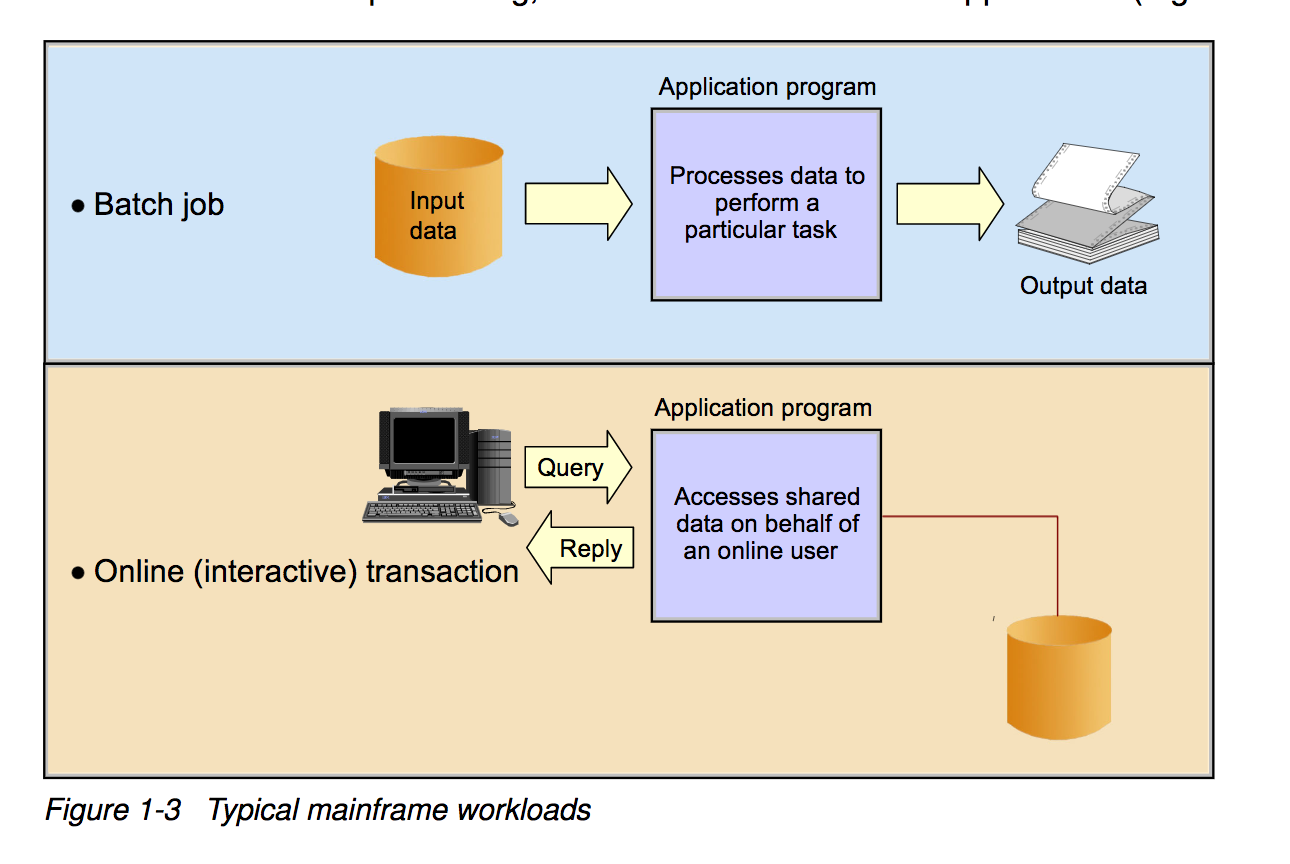
\includegraphics[scale=0.5]{img/batchtrans.png}
	\caption{Typical workloads}
	\label{Typical workloads}
\end{figure}
\ \\
\subsection{Online Transaction Processing}
One of the core functions of many businesses is OLTP. For this case the mainframe serves a large amount of applications to make it possible to execute thousands of transactions in short time while handling not only a huge amount of different transaction types, but also to do this with many different users at a glance.\\
For end-users those transaction processes are often commonly known, while they appear in everyday's life, such as:
\begin{itemize}
\item Credit card payments in supermarkets
\item ATM transactions
\item Online purchasings
\end{itemize}

\textbf{---- Explain Online part and why not consolidated in this thesis ---- }

\subsection{Batch Processing}
The other main function of the mainframe is processing data in a batch. Eventually terabytes of. These processes are generally done without much user interaction. A batch job simply gets committed and processes the data that is determined in the job-statement ( further informations in chapter \ref{JCL} )

\textit{ An 
equivalent concept can be found in a UNIX script file or a Windows command 
file, but a z/OS batch job might process millions of records.}\\

\textbf{---- Explain deeper and bridge to System Operators ---- }


\ \\
\subsection{Separation of duties}
distinguish between:
\begin{itemize}
\item System programmers 
\item System administrators (for example, DBA, storage, network, security, and 
performance)
\item Application designers and programmers 
\item \textbf{System operators (explain)}
\item Production control analysts
\end{itemize}
\ \\
\subsection{Mainframe Operation Systems}
z/OS\\
z/VM\\
z/VSE\\
Linux for zSeries\\
z/TPF\\
\ \\

\subsection{Virtualisation with z/VM}
\textit{As an aid to consolidation, the mainframe offers software virtualization, through z/VM. z/VM?s extreme virtualization capabilities, which have been perfected since its introduction in 1967, make it possible to virtualize thousands of  distributed servers on a single server, resulting in the significant reduction in the use of space and energy. }
\ \\
\textit{z/Virtual Machine (z/VM) has two basic components: a control program (CP) and 
a single-user operating system (CMS). As a control program, z/VM is a hypervisor because it runs other operating systems in the virtual machines it creates. Any of the IBM mainframe operating systems such as z/OS, Linux on System z, z/VSE, and z/TPF can be run as guest systemsin their own virtual machines, and z/VM can run any combination of guest systems.}\\
\textbf{---- Explain and show z/VM Constellation, LPARs etc ---- }
\ \\
more in : \url{http://www.redbooks.ibm.com/redbooks/pdfs/sg247603.pdf}
\newpage


%================== Research Gap ===========================%


\section{Research gap}
While the web-access to z/OS for OLTP is very established because of the usage, that is often conducted by end-users or computers, that are not located in immediate proximity to the server, the access to the JES-spool through web-applications is less common, since the system-operators are usually working in ultimate contact to the mainframe.\\
Certainly there are operators handling batch-processes through a web front-end due to flexibility and simplicity reasons. But while these applications are to simplify the process of managing the workload in daily-business, this thesis tries to establish an environment where the jobs have to be done in full amplitude, but on a test-system, implemented just for educational reasons.\\
This setup will have the ambitions of getting people into JCL quite quickly on the one hand and give them the opportunity to train their abilities and, in this way reduce potential uncertainties towards working on large-scale systems, on the other hand. With this method a pertinent and long-lasting learning effect is to be achieved in short time.\\
\newpage


%================== JCL ===========================%


\section{Dive into \ac{JCL}}
\label{JCL}
\textbf{---- Important to understand JCL for accessing JES Spool?! ---- }\\
\ \\
To get familiar with JCL, this chapter will give an introduction in how these Statements are working. There is talk about "Statements", because JCL is used to tell the OS what to do. Each Statement is an independent work unit, known as "Job" - therefore this language is called "Job Control Language". Each Job consists of instructions that are either typed in by an operator or they are stored and get transmitted to the computer. \\ 

\subsection{Job Control Environment}
So to understand how a job is executed, it is important to know which components are needed for this process.\\
\begin{figure}[h]
	\centering
	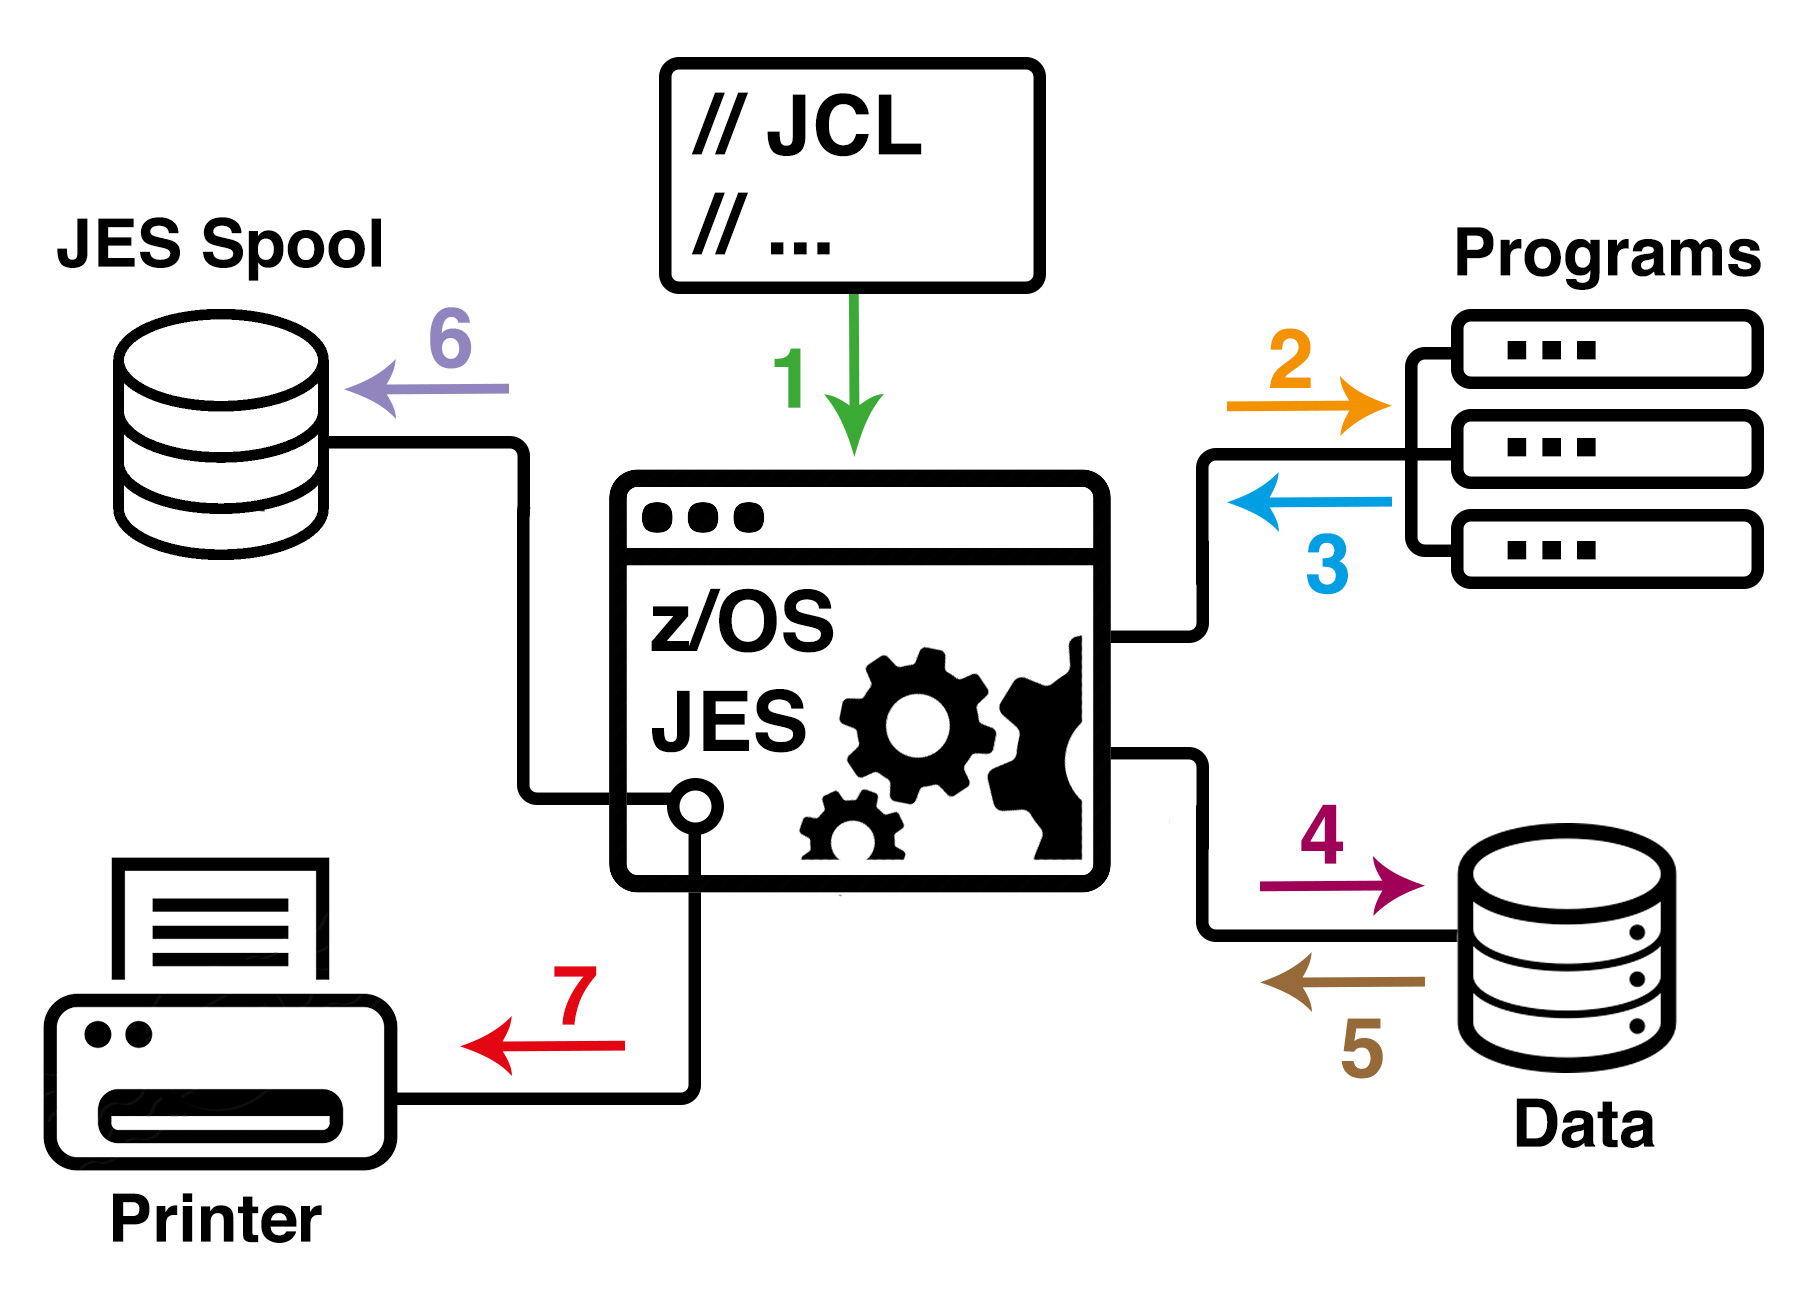
\includegraphics[scale=0.25]{img/JCL-1.jpg}
	\caption{JCL Functionality, Source: IBM}
	\label{JCL Functionality}
\end{figure}
\ \\
On figure \ref{JCL Functionality} you can see a job process described in 7 steps.\\
\begin{enumerate}
\item JCL submit 
\item JCL requests program 
\item Program gets loaded
\item Resources for program get allocated through JCL
\item Resources get provided to program
\item Program writes output to JES Spool
\item Output to gets transferred to printer as requested
\end{enumerate}
\ \\
The z/OS has written (hard coded) application programs which are not associated with any physical resources. Those programs are just names, which include internal file-names. Through JCL those programs can be opened for reading and writing during execution.\\
The \ac{JES} is there to evaluate and accept or not accept a job. If the syntax is right and the job is accepted the JES runs it on the OS and controls this process. The results get transferred to an output unit.\\


\subsection{Job structure}
-each statement 80characters\\
-JCL is introduced with // \\

\subsubsection{EXEC-Statements}
Within a job, there are working executions introduced through an "EXEC-statement". Every job needs at least one execution, but there can obviously be many more in addition. If a job has no execution it stops.
\ \\
\begin{lstlisting}[language=PHP]
//STEP0001 EXEC PGM=IEBGENER
...
//STEP0002 EXEC PROC=PRDPROC1
//STEP0003 EXEC PRDPROC2
\end{lstlisting}


\subsubsection{DD-Statements}
\begin{itemize}
\item{SYSUT1}
\item{SYSUT2}
\item{SYSIN}
\item{SYSPRINT}
\end{itemize}
-JCL links the program file names with physical resources (e.g. data set names or unix file names).\\
--JCL is used to process programs in the background ("batch")\\
- And to process programs in the foreground("started task")\\
-JCL instruct z/OS -> Start / submit
- JCL SUBMIT Statement will result in batch process of one or more programs (BACKGROUND)\\
- JCL START will result in FOREGROUND processing of a processing program\\
\ \\
\subsubsection{Background / Foreground jobs}
Every Batch Job must contain JOB-statement \& EXEC statement\\
->JOB statement highlight the beginning of a batch job \& assigns a name to the job\\
JCL started tasks do not require a JOB Statement
->both have at least one EXEC statement -> marks the beginning of a job step , assigns name to the step \& identifies the program or procedure to be executed in the step.

\newpage



%================== Get Access to JES ===========================%



\section{Access possibilities}
In order to execute JCL-Jobs on z/OS from the Linux host, an access point is required to submit the data. This chapter is to reveal how the z/VM connects the Linux-host and the z-OS Target-system in this case and how this connection can be used to transfer data among them.\\
To enable the communication between different applications, a protocol is needed. The protocol that is used in the System Z is the \ac{TCP}/\ac{IP}, which is provided through the HiperSockets function. HiperSockets is a technology developed by IBM to enable high-speed communication between \ac{LPAR} with a hypervisor or between applications inside a z/VM as it is the case here.\\
You could imagine a HiperSockets-network like an internal \ac{LAN}, linking all partitions for internal communication.\\
\begin{figure}[h]
	\centering
	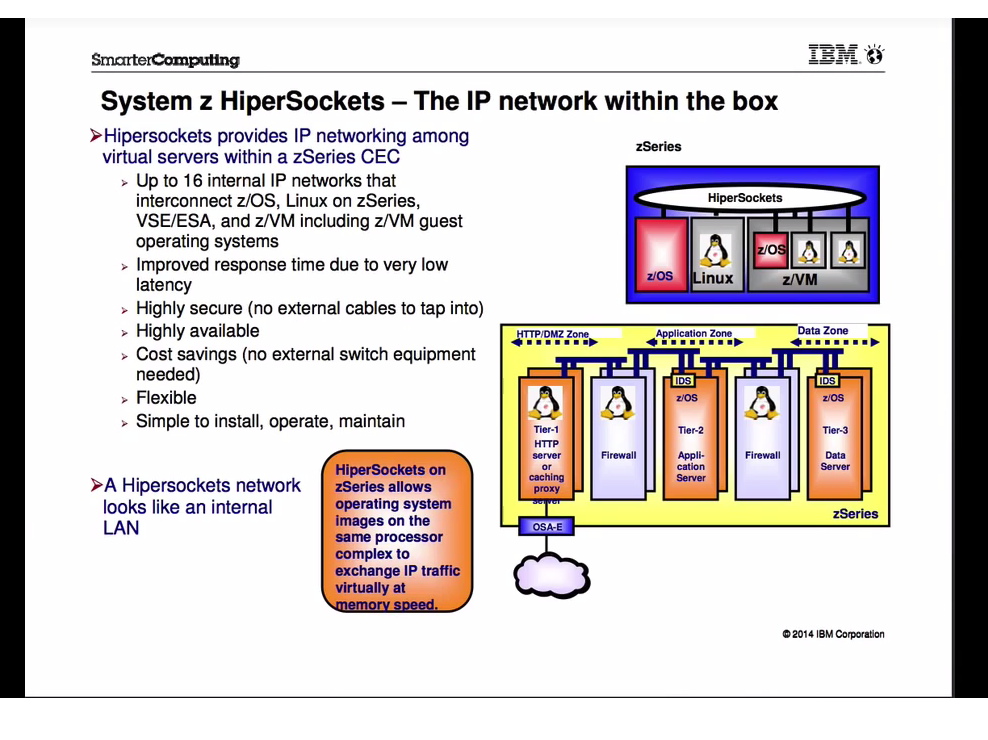
\includegraphics[scale=0.7]{img/Hiper.png}
	\caption{TCP/IP Connection / Hipersockets}
	\label{Hipersockets}
\end{figure}
\ \\
\begin{figure}[h]
	\centering
	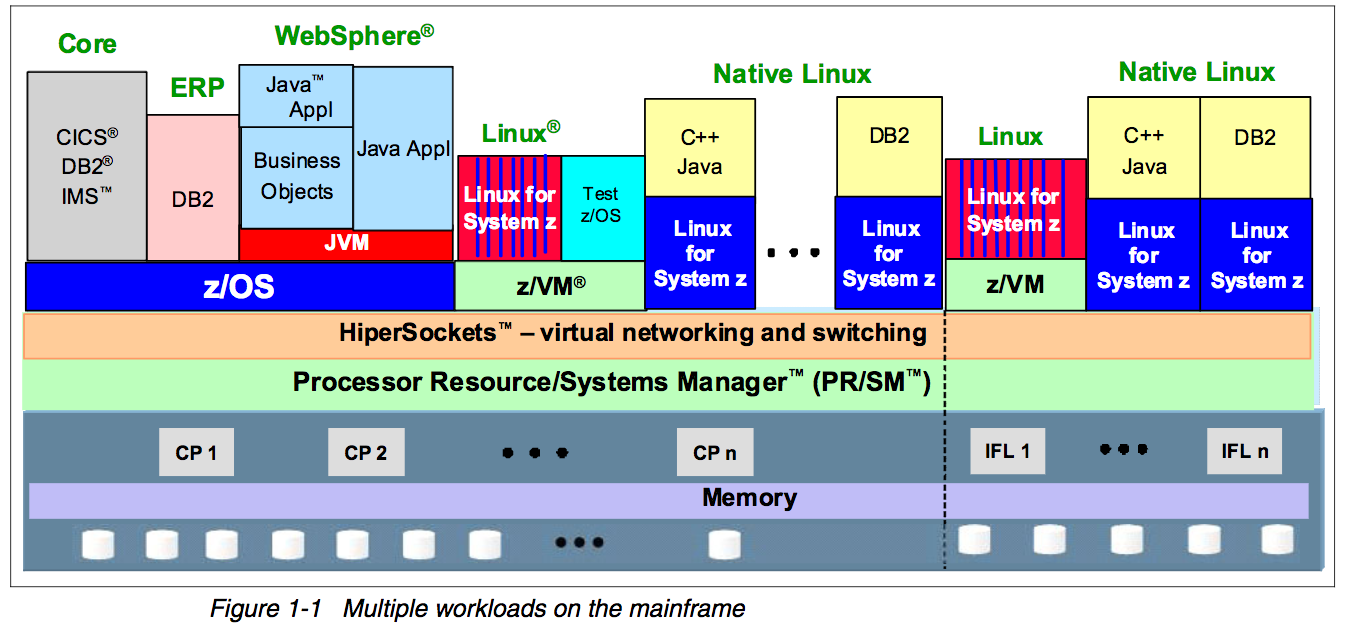
\includegraphics[scale=0.7]{img/workloads.png}
	\caption{workloads}
	\label{workloads}
\end{figure}

\textbf{---- Explain Hipersockets / TCP/IP Connection ---- }\\
A way we can use this connection to transfer jcl-jobs is:
\ \\
\begin{myboxii}[Transmission Control Protocol]
The Transmission Control Protocol (TCP) provides a reliable vehicle for delivering
packets between hosts on an internet. TCP takes a stream of data, breaks it into
datagrams, sends each one individually using IP, and reassembles the datagrams at
the destination node. If any datagrams are lost or damaged during transmission,
TCP detects this and resends the missing datagrams. The received data stream is a
reliable copy of the transmitted data stream.

\textbf{---- Explain TCP/IP Connection in own words ---- }\\

\end{myboxii}
\ \\
\subsection{Access through Java with FTP}
What becomes possible through the TCP/IP in System Z is the \ac{FTP} Server, an IP-application used to transfer files between any kind of platform. The z/OS FTP-Server is a bit different from normal FTP-Servers as it provides not only the possibility to transfer files and get access to z/OS System Services, but it also provides access to the Job Entry Subsystem which is, as mentioned in  chapter \ref{JCL}, needed to submit JCL-Jobs.\\

With the help of Java you can use the FTP server to get access to a number of JES functions, including the following:
\begin{itemize}
\item Submitting a job
\item Displaying the status of jobs
\item Receiving the spool output of a job (JCL messages and SYSOUT)
\item Deleting a job
\item Submitting a job and automatically receiving output
\end{itemize}
\ \\
\textbf{---- Importance of output for Learning environment ---- }\\

\subsection{Access via \ac{SSH}/ \ac{SFTP}}
While FTP gives us the opportunity to get access to the JES-Spool to run JCL-Jobs, this is not really a safe way to work this out.\\
To get a safe communication, it needs encryption what can be established through the SSH-protocol - making the FTP a Secure File Transfer Protocol.\\

\begin{myboxii}[The Secure Shell Protocol]
The SSH protocol (also referred to as Secure Shell) is a method for secure remote login from one computer to another. It provides several alternative options for strong authentication, and it protects the communications security and integrity with strong encryption. It is a secure alternative to the non-protected login protocols (such as telnet, rlogin) and insecure file transfer methods (such as FTP). 
\textbf{---- Explain SSH in own words ---- }\\

\end{myboxii}

\newpage

%================== Requirements and Development ===========================%


\section{Requirements}
A tool named Co:Z SFTP, an open-source product developed by Dovetail Technologies, will help to establish a safe connection with before mentioned techniques. It works as a port of OpenSSH SFTP for z/OS and therefore enables the access to z/OS datasets and spool files.\\

\url{http://www.redbooks.ibm.com/redbooks/pdfs/sg247603.pdf}
from p.137
\newpage


\section{Development Environment}
In this chapter, a development environment will be created. An Oracle Virtual-Machine called VirtualBox will be installed on MacOSX. In this virtual machine the open and free Linux-System Ubuntu 16.04 LTS will be running, to make it possible to implement an Apache HTTP-Server. The Apache Server makes it possible to develop a simple dynamic website offline on a localhost that can be accessed through any web-browser as long as the virtual machine is running.\\
\\Schematische Darstellung!!

\ \\
Electron Framework short explanation\\


\newpage


\section{Design}
We use a one-page Framework (hyperspace ansprechen?!) \\
Co:Z Documentation can be visited on \hyperlink{http://dovetail.com/docs/sftp/using.html}{http://dovetail.com/docs/sftp/using.html}\\
Implementation of 4 sections: \\
\subsection{Welcome}
Not much explanation needed - Get started leads to first section: Your Jobs.
Perhaps gamification part with points/stars or something.
For use of the next sections an SFTP-Client is implemented to get a connection to Co:Z-SFTP\\
ssh2.js library explanation?!\\

\begin{lstlisting}[language=Java]
var Client = require('ssh2').Client;
var connection = new Client();

var connSettings = {
     host: '141.2.192.32',
     port: 22, // Guest-SFTP Port
     username: 'u0xxx',
     password: 'xxxxxxxx'
};
\end{lstlisting}

\subsection{Your Jobs}
In this section the user can see the jobs he or she submitted so far and in addition the job the user is currently working on.\\
\begin{lstlisting}[language=HTML]
       <!-- Here the JES-Spool is listed -->
       <div id="dirout"></div>
\end{lstlisting}

With the following JS-function, the jobs are passed to the application.\\
\begin{lstlisting}[language=Java]
var remotePathToList = '//-JES';

var conn = new Client();
conn.on('ready', function() {
    conn.sftp(function(err, sftp) {
         if (err) throw err;

         sftp.readdir(remotePathToList, function(err, list) {
                if (err) throw err;

                var rows = list;

                    var jobs = "<table border='1|1'>";
                    for (var i = 0; i < rows.length; i++) {
                        jobs+="<tr>";
                        jobs+="<td>"+rows[i].filename+"</td>";
                        jobs+="<td>"+rows[i].longname+"</td>";

                        jobs+="</tr>";
                    }
                    jobs+="</table>";
                document.getElementById("dirout").innerHTML = jobs;

                // Do not forget to close the connection, otherwise you'll get troubles
                conn.end();
         });
    });
}).connect(connSettings);
\end{lstlisting}
\ \\
\begin{itemize}
\item{Line 1: Navigating to the //-JES directory, which is a directory, defined through Co:Z and contains the job-files.}
\item{Lines 3-5: Here the connection is established with the above described parameters.}
\item{Line 6: Throws an error if something went wrong (in console! to be changed?!).}
\item{from Line 8: the directory is readed. Here two variables, err and list, are defined. The err variable is just to get output in case of errors. List defines the Objects located in the //-JES directory. }
\item{from Line 11: The List content gets defined as rows, those rows are given to a table that is defined as a variable "jobs". The function in jobs, adds a row for each object.}
\item{Line 22: Calls a div in index.html with the id="dirout" which is empty by default. Here it puts the table with the listed jobs.}
\item{After this the connection is ended, to get always just a status of the directory in the moment it is charged.}
\end{itemize}

\subsection{Submit a new Job}
First a file is created as a text-file. explain buttons.\\
Screenshots!?\\
\begin{lstlisting}[language=HTML]
          <button onclick="createFile()">Create Job</button>
\end{lstlisting}
\ \\
\begin{lstlisting}[language=HTML]
   <div style="margin-top:30px;">
     <p id="filesuccess">Write your Job in the textarea above and 
     		click on Create Job.</p>
     <div class="field">
       <button id="subBut" style="display:none;" onclick="transFile()">
       			Submit the Job now</button>
       <div id="messages"></div>
     </div>
   </div>
\end{lstlisting}
\ \\
Use node filesystem. Change content - innerHTML and color. explain variables.
\begin{lstlisting}[language=Java]
// Create Job file
function createFile() {
  var fs = require('fs');
  var filepath = "temp/JCL.txt";
  var fileContent = document.getElementById("JCLcontent").value;
  var filesuccess = document.getElementById("filesuccess");
  var subBut = document.getElementById("subBut");

  //Check if textarea contains content
  if (fileContent == '') {

    filesuccess.style.color = "#ff9800";
    filesuccess.innerHTML = "Please write a Job first.";

  } else if (fileContent != '') {

    // if it does, create textfile
    fs.writeFile(filepath, fileContent, (err) => {
                    if (err) throw err;

      //output as success or "create a job first"
      filesuccess.style.color = "#00e676";
      filesuccess.innerHTML = "Your Job has been created. 
      			Submit now to the JES-Spool.";
      subBut.style.display = "block";

        });
  }
};
\end{lstlisting}
\ \\
Change the mode ls = readdir in node. Explain streams. 
\begin{lstlisting}[language=Java]
//Transfer Job File to Mainframe
function transFile() {
var changeMod = '/+mode=text'

var conn = new Client();
  conn.on('ready', function() {
    console.log('Client -> ready');
      conn.sftp(function(err, sftp) {
           if (err) throw err;

             // change Transfer Mode with ls /+mode=text
             sftp.readdir(changeMod, function(err, list) {
                    if (err) throw err;
                    // List the Changing in the console
                    console.dir('mode -> text');
                    // This time no connection closing, to get the output-action
             });


             var fs = require("fs"); // Use node filesystem
             
             //Read the textfile and send it to subdirectory, called "myjob"
             var readStream = fs.createReadStream( 'temp/JCL.txt' );
             var writeStream = sftp.createWriteStream( '//-JES.INTRDR/MYJOB' );

             writeStream.on('close',function () {
                 console.log( "file transferred succesfully" );
                 document.getElementById('three').style.display = 'block';
             });

             writeStream.on('end', function () {
                 console.log( "sftp connection closed" );
                 conn.close();
             });

             // initiate transfer of file
             readStream.pipe( writeStream );
         });

      }).connect(connSettings);
  };
\end{lstlisting}
\ \\
"three" = Result area -> gets displayed after submitting
\subsection{Result}
Here describe Error handling and output divs.


\begin{lstlisting}[language=Java]
<section id="three" class="wrapper style3 fade-up">

   <div class="inner">
      <h2>Your Result</h2>
      <p>Here you can see if your job was submitted to the mainframe. 
      To get more details on the job status go to the overview. 
      You can also check the return code there.</p>
      
  <div class="features">
  <section id="resultinfo">
      <span class="icon major fa-info"></span>
      <h3>No submit</h3>
      <p>You first have to submit something to get a result.</p>
  </section>
  
   <section id="goodresult" style="display:none;">
      <span class="icon major fa-check"></span>
      <h3>You succeeded</h3>
      <p>Your file was submitted. 
      Go to the overview to check its status.</p>
   </section>
   
   <section id="badresult" style="display:none;">
     <span class="icon major fa-times"></span>
     <h3>Something went wrong</h3>
     <p>Bad Connection. Check your VPN.</p>
   </section>
   </div>
   
   // The page has to get reloaded to view the new jobs in the list 
     <ul class="actions">
       <li><a href="#one" class="button" 
       	onClick="window.location.reload()">Go to overview</a></li>
     </ul>
     
   </div>
 </section>
\end{lstlisting}
Catch TimeOut Error in ssh2 library, Client function.
\begin{lstlisting}[language=Java]
function Client() {

 [ ... ]
 
   function startTimeout() {
    if (self.config.readyTimeout > 0) {
      self._readyTimeout = setTimeout(function() {
        var err = new Error('Timed out while waiting for handshake');

        document.getElementById("badlist").style.display = "block";
        document.getElementById("resultinfo").style.display = "none";
        document.getElementById("badresult").style.display = "block";

        err.level = 'client-timeout';
        self.emit('error', err);
        sock.destroy();
      }, self.config.readyTimeout);
    }
  }
};
\end{lstlisting}

\newpage
\section{Proof of Concept}
\section{Evaluation}

\newpage





%\end{onehalfspacing}

\newpage
\bibliographystyle{plain}
\bibliography{bibfile}


\newpage
\section{Appendices}






\end{document}